\documentclass[11pt]{article}

\usepackage{float}
\usepackage{hyperref}
\usepackage{graphicx}
% formatting
\usepackage{verbatim}
\usepackage{moreverb}
\usepackage{minted}
\usepackage{parskip}
\usepackage{amsmath}
\usepackage[listings]{tcolorbox}
\usepackage{enumerate}
\usepackage{tikz}
\usetikzlibrary{arrows,automata, positioning}
\let\verbatiminput=\verbatimtabinput
\def\verbatimtabsize{4\relax}

\newcommand{\RepoRootPath}{fpga\_labs\_fa19}

\tcbset{
texexp/.style={colframe=black, colback=lightgray!15,
         coltitle=white,
         fonttitle=\small\sffamily\bfseries, fontupper=\small, fontlower=\small},
     example/.style 2 args={texexp,
title={Question \thetcbcounter: #1},label={#2}},
}

\newtcolorbox{texexp}[1]{texexp}
\newtcolorbox[auto counter]{texexptitled}[3][]{%
example={#2}{#3},#1}

\setlength{\topmargin}{-0.5in}
\setlength{\textheight}{9in}
\setlength{\oddsidemargin}{0in}
\setlength{\evensidemargin}{0in}
\setlength{\textwidth}{6.5in}

% Useful macros

\newcommand{\note}[1]{{\bf [ NOTE: #1 ]}}
\newcommand{\fixme}[1]{{\bf [ FIXME: #1 ]}}
\newcommand{\wunits}[2]{\mbox{#1\,#2}}
\newcommand{\um}{\mbox{$\mu$m}}
\newcommand{\xum}[1]{\wunits{#1}{\um}}
\newcommand{\by}[2]{\mbox{#1$\times$#2}}
\newcommand{\byby}[3]{\mbox{#1$\times$#2$\times$#3}}


\newenvironment{tightlist}
{\begin{itemize}
 \setlength{\parsep}{0pt}
 \setlength{\itemsep}{-2pt}}
{\end{itemize}}

\newenvironment{titledtightlist}[1]
{\noindent
 ~~\textbf{#1}
 \begin{itemize}
 \setlength{\parsep}{0pt}
 \setlength{\itemsep}{-2pt}}
{\end{itemize}}

% Change spacing before and after section headers

\makeatletter
\renewcommand{\section}
{\@startsection {section}{1}{0pt}
 {-2ex}
 {1ex}
 {\bfseries\Large}}
\makeatother

\makeatletter
\renewcommand{\subsection}
{\@startsection {subsection}{1}{0pt}
 {-1ex}
 {0.5ex}
 {\bfseries\normalsize}}
\makeatother

% Reduce likelihood of a single line at the top/bottom of page
\clubpenalty=2000
\widowpenalty=2000

% Other commands and parameters
\pagestyle{myheadings}
\setlength{\parindent}{0in}
\setlength{\parskip}{10pt}

% Commands for register format figures.
\newcommand{\instbit}[1]{\mbox{\scriptsize #1}}
\newcommand{\instbitrange}[2]{\instbit{#1} \hfill \instbit{#2}}

\begin{document}

\def\PYZsq{\textquotesingle}
\title{\vspace{-0.4in}\Large \bf EECS 151/251A FPGA Lab 4:\\Memories, IO Circuits, FSMs\vspace{-0.1in}}

\author{Prof. Borivoje Nikolic and Prof. Sophia Shao \\
TAs: Cem Yalcin, Rebekah Zhao, Ryan Kaveh, Vighnesh Iyer \\ Department of Electrical Engineering and Computer Sciences\\
College of Engineering, University of California, Berkeley}
\date{}
\maketitle

\newcommand{\headertext}{EECS 151/251A FPGA Lab 4: Memories, IO Circuits, FSMs}
\markboth{\headertext}{\headertext}
\thispagestyle{empty}

\section{Before You Start This Lab}
Run \verb|git pull| in \texttt{\RepoRootPath}.

Review these documents that will help you better understand some concepts we will be covering.

\begin{enumerate}
  \item \href{http://inst.eecs.berkeley.edu/~eecs151/fa19/files/verilog/verilog_fsm.pdf}{verilog\_fsm.pdf} - constructing FSMs in Verilog.
  \item \href{http://www.labbookpages.co.uk/electronics/debounce.html}{Debouncer Circuit}

  Read the ``What is Switch Bounce'' section to get idea of why we need a debouncer circuit. Read the ``Digital Switch Debouncing'' section to get a general overview of the circuit, its parts, and their functions.
\end{enumerate}

\section{Lab Overview}
In this lab, we will
\begin{itemize}
  \item use a ROM to store a melody and play it on the FPGA using the \verb|tone_generator|
  \item build input conditioning circuits that make control signals from physical input devices, like the buttons and switches we've been using up to now, more reliable
  \item verify the conditioning circuits are working correctly using the FPGA LEDs
  \item use synchronous resets to reset our circuits to a known initial state
  \item create a basic FSM in the \verb|music_streamer| that uses the buttons to change states and alter the music playback
  \item (optionally) extend our \verb|music_streamer| into a sequencer.
\end{itemize}

\section{Using an Asynchronous ROM to Build the Music Streamer}
An asynchronous memory is a memory block that isn't governed by a clock. In this lab, we will use a Python script to generate a ROM block in Verilog.

A ROM is a read-only memory. This data can be accessed by supplying an address to the ROM; after some time, the ROM will output the data stored at that address. A memory block in general can contain as many addresses in which to store data as you desire. Every address should contain the same amount of data (bits). The number of addresses is called the \textbf{depth} of the memory, while the number of bits stored per address is called the \textbf{width} of the memory.

The synthesizer takes the Verilog you write and converts it into a low-level netlist of the structures are actually used on the FPGA. Our Verilog \textbf{describes} the functionality of some digital circuit and the synthesizer \textbf{infers} what primitives implement the functional description. In this section, we will examine the Verilog that allows the synthesizer to infer a ROM. This is a minimal example of a ROM in Verilog: (depth of 8 entries/addresses, width of 12 bits)

\begin{minted}[tabsize=2]{verilog}
module rom (input [2:0] address, output reg [11:0] data);
  always @(*) begin
    case(address)
      3'd0: data = 12'h000;
      3'd1: data = 12'hFFF;
      3'd2: data = 12'hACD;
      3'd3: data = 12'h122;
      3'd4: data = 12'h347;
      3'd5: data = 12'h93A;
      3'd6: data = 12'h0AF;
      3'd7: data = 12'hC2B;
    endcase
  end
endmodule
\end{minted}

To power our \verb|tone_generator|, we will be using a ROM that is X entries/addresses deep and 24 bits wide. The ROM will contain tones that the \verb|tone_generator| will play. You can choose the depth of your ROM based on the length of the sequence of tones you want to play.

We've provided you with a few scripts that can generate a ROM from either a file with it's contents or even from sheet music. Run these commands from \verb|lab3/|.

\begin{minted}{bash}
python scripts/musicxml_parser.py musicxml/Twinkle_Twinkle_Little_Star.mxl music.txt
python scripts/rom_generator.py music.txt ./lab3.srcs/sources_1/new/rom.v 1024 24
\end{minted}

The first script will parse a MusicXML file and turn it into a list of \verb|tone_switch_periods| for each of the notes for a piece of sheet music. The second script will take that list and turn it into a ROM that's 1024 entries deep with a width of 24 bits.

Take a look at \verb|music.txt| and \verb|src/rom.v|. You can download your own music in MusicXML format from here (\url{https://musescore.org/}) and run it through the same parser; it should ideally only have one part to work properly. You can also directly edit the \verb|music.txt| file to customize the contents of the ROM as you wish.

\section{Design of the music\_streamer}
Open up the \verb|music_streamer.v| file. You will need to modify this module to contain an instance of the ROM you created earlier and logic to address the ROM sequentially to play notes. The \verb|music_streamer| will play each note in the ROM for a predefined amount of time by sending it to the \verb|tone_generator|.

We will play each note for 1/25th of a second. Calculate what that is in terms of 125Mhz clock cycles.

Now let's begin the design of the \verb|music_streamer| itself. Instantiate your ROM in the \verb|music_streamer| and connect the ROM's \verb|address| and \verb|data| ports to wire or reg nets that you create in your module.  The \verb|last_address| port outputs the last address in the ROM (depth).

Next, write the RTL that will increment the address supplied to the ROM every \textbf{1/25th of a second}. The data coming out of the ROM should be fed to the \verb|tone| output. The ROM's address input should go from 0 to the depth of the ROM and should then loop around back to 0. You don't have a reset signal, so define the initial state of any registers in your design for simulation purposes. Also hook up the \verb|rom_address| output to the ROM address currently being accessed.

Now that you have implemented \verb|music_streamer|, create an instance of it in the module \verb|z1top.v|. Use the instance name \verb|streamer| to match the expected name in the \verb|.do| file. Instantiate a \verb|tone_generator| and wire \verb|SWITCHES[1]| to \verb|output_enable|, \verb|CLK_125MHZ_FPGA| to \verb|clk|, and \verb|aud_pwm| to \verb|square_wave_out|.  Assign \verb|aud_sd| to 1.  Connect the \verb|tone| output of the \verb|music_streamer| to the \verb|tone_switch_period| input of the \verb|tone_generator|. Connect the \verb|music_streamer|'s \verb|clk| input to the global clock signal. Finally, connect  its \verb|rom_address| output to the \verb|LEDS|s by routing the top 6 bits of address.

\section{Testbench Techniques} \label{sec:testbenchtechniques}
There are several testbenches included in this lab for your synchronizer, edge detector, shift register, debouncer, and music streamer that introduce you to some useful Verilog testbench constructs.

\begin{itemize}
\item \verb|@(posedge <signal>)| and \verb|@(negedge <signal>)| - These are a different type of delay statement from what you have seen before. \verb|#10| would advance the simulation by 10 timesteps. These commands will advance the simulation until the \verb|<signal>| rises or falls.

For example:
\begin{minted}[frame=single]{verilog}
@(posedge signal);
@(posedge signal);
\end{minted}

Simulation time will advance until we have seen two rising edges of \verb|signal|.

\item \verb|repeat| - it acts like a \verb|for| loop but without an increment variable

For example:
\begin{minted}[frame=single, tabsize=4]{verilog}
repeat (2) @(negedge clk);
repeat (10) begin 
	@(posedge clk);
end
\end{minted} 

The simulation will advance until we have seen 2 falling clock edges and will then advance further until we have seen 10 rising clock edges.

\item \verb|$display| - acts as a print statement. Similar to languages like C, if you want to print out a wire, reg, integer, etc... value in your testbench, you will need to format the string. It works like \verb|printf()| in C.

For example:
\begin{minted}[frame=single]{verilog}
$display("Wire x in decimal is %d", x);
$display("Wire x in binary is %b", x);
\end{minted} 

\item \verb|tasks| - tasks are subroutines where you can group and organize some commands rather than haphazardly putting them everywhere. They can take inputs and assign outputs. 

\begin{minted}[frame=single, tabsize=4]{verilog}
task wait_for_n_clocks();
input [7:0] num_edges;
begin
	repeat (num_edges) @(posedge clk);
end
endtask
\end{minted}

\item \verb|fork/join| - Allows you to execute testbench code in parallel. You create a fork block with the keyword \verb|fork| and end the block with the keyword \verb|join|.

For example:
\begin{minted}[frame=single, tabsize=4]{verilog}
fork
	begin
		task1();
	end
	begin
		$display("Another thread");
		task2();
	end
join
\end{minted}

Multiple threads of execution are created by putting multiple begin/end blocks in the fork-join block. In this example, thread 1 runs \verb|task1()|, while thread 2 first \verb|$display|s some text then runs \verb|task2()|. The threads operate in parallel.

\item Hierarchical Paths - you can access signals inside an instantiated module for debugging purposes. This can be helpful in some cases where you want to look at an internal signal but don't want to create another output port just for debug.

For example:
\begin{minted}[frame=single, breaklines]{verilog}
tone_generator tone_gen ();
$display("Signal inside my tone_generator instance, clock_counter: %b", tone_gen.clock_counter);
\end{minted} 
\end{itemize}


\section{Simulating the music\_streamer}
To simulate your \verb|music_streamer| open up the \verb|lab3/src/music_streamer_testbench.v|. In contrast to the \verb|tone_generator_testbench| where the \verb|tone_generator| was instantiated in isolation, in this testbench we are instantiating our entire top-level design, \verb|z1top|. This testbench is referred to as a system-level testbench, which tests our entire design using top-level I/O, in contrast to the \verb|tone_generator_testbench| which is a block-level testbench. This is similar to the difference between unit and integration tests in software development.

You can see that this testbench just runs a simulation for 2 seconds and then exits. You might have to modify the \verb|music_streamer_testbench.do| file to match the name of your module instances in \verb|z1top.v|.

To execute the testbench, run \verb|make CASES=tests/music_streamer_testbench.do| in \verb|lab3/sim|. This may take several minutes to complete. You may have to run \verb|make clean| before running \verb|make| if ModelSim has cached build artifacts.

Inspect your waveform to make sure you get what you expect. Verify that there are no undefined signals (red lines, x) Then run the Python script to generate a \verb|.wav| file of your simulation results and listen to your \verb|music_streamer|. It should sound like the first few seconds of the song that was loaded on the ROM.

\section{Verify your Code Works For Rest Notes}
In simulation, you can often catch bugs that would be difficult or impossible to catch by running your circuit on the FPGA. You should verify that if your ROM contains an entry that is zero (i.e. generate a 0Hz wave), that the \verb|tone_generator| holds the \verb|square_wave_out| output at either 1 or 0 with no oscillation. Verify this in simulation, and prove the correct functionality during checkoff.

\section{Try it on the FPGA!}
Now try your \verb|music_streamer| on the FPGA. You should expect the output to be the same as in simulation. The \verb|SWITCHES[1]| switch should still work to disable the output of the \verb|tone_generator|. Show your final results, simulation, and the working design on the FPGA to the TA for checkoff.

\section{Synchronizer, Debouncer}

\subsection{Synchronizer}
In Verilog (RTL), digital signals are either 0's or 1's. In a digital circuit, a 0 or 1 corresponds to a low or high voltage. If the circuit is well designed and timed (fully synchronous), we only have to worry about the low and high voltage states, but in this lab we will be dealing with asynchronous signals.

The signals coming from the push buttons and slide switches on the PYNQ-Z1 board don't have an associated clock signal. For the push-buttons in particular, when those signals are put through a register, the hold or setup time constraints of that register may be violated. This may put that register into a \textbf{metastable} state.

\begin{figure}[H]
	\centerline{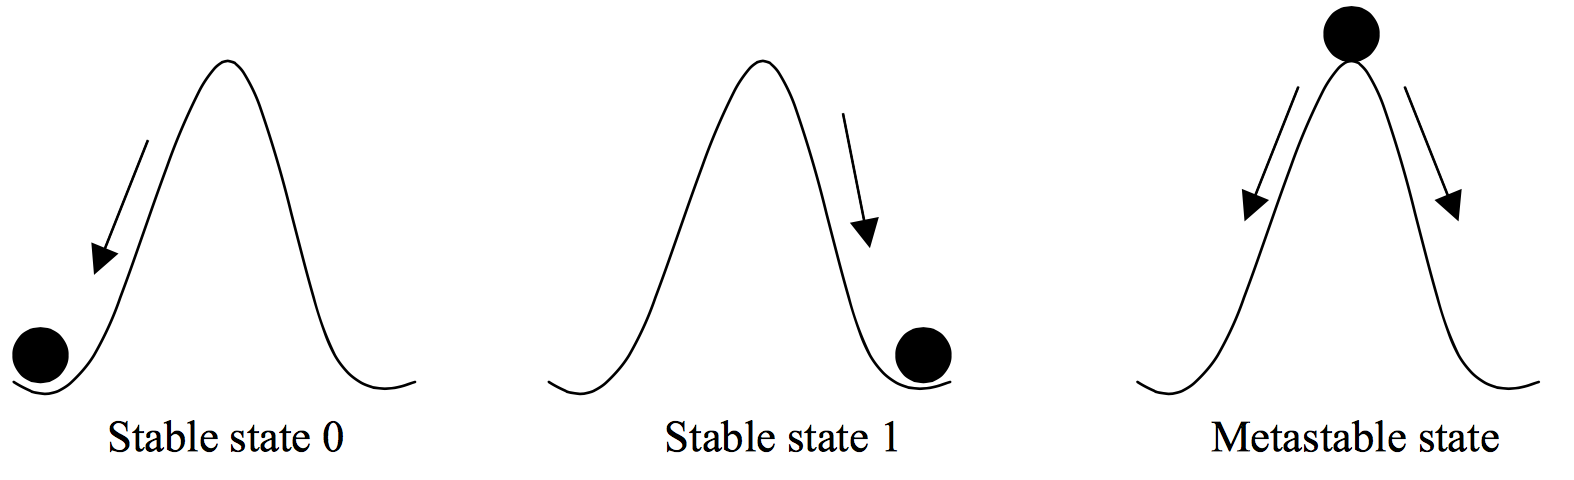
\includegraphics[height=3cm]{figs/lab2_fig3.png}}
	\caption{The `ball on a hill' metaphor for metastability. If a register's timing constraints are violated, its output voltage oscillates and after some time unpredictably settles to a stable state.}
\end{figure}

In a fully synchronous circuit, the timing tools will determine the fastest clock frequency under which the setup time constraints are all respected and the routing tools will ensure that any hold time constraints are handled. Introducing an asynchronous signal that isn't changing with respect to a clock signal can cause a register to go into a metastable state. This is undesirable since this will cause a `mid-rail' voltage to propagate to other logic elements and can cause catastrophic timing violations that the tools never saw coming.

We will implement a synchronizer circuit that will safely bring an asynchronous signal into a synchronous circuit. The synchronizer needs to have a very small probability of allowing metastability to propagate into our synchronous circuit.

This synchronizer circuit we want you to implement for this lab is relatively simple. For synchronizing one bit, it is a pair of flip-flops connected serially. This circuit synchronizes an asynchronous signal (not related to any clock) coming into the FPGA. We will be using our synchronizer circuit to bring any asynchronous off-FPGA signals into the clock domain of our FPGA design.

\begin{figure}[H]
	\vspace{0.5cm}
	\centerline{\includegraphics[height=2.5cm]{figs/Synchronizer.png}}
	\caption{1-bit 2 Flip-Flop Synchronizer}
\end{figure}

Edit the \verb|synchronizer.v| (in your project sources) file to implement the two flip-flop synchronizer. This module is parameterized by a \verb|width| parameter which indicates the number of one-bit signals to synchronize.

\subsubsection{Testing in Simulation}
The testbenches to be run are stored in \verb|lab4/sim/tests|. Each \verb|.do| file in this directory is run when you run \verb|make| in the \verb|lab4/sim| directory. If you only want to run one testbench, you can rename all the other \verb|.do| files in this directory to have a different file extension. Alternatively, you can leave the file extensions alone, and specify the test you want to run like this:

\begin{minted}{bash}
cd lab4/sim
make CASES="tests/sync_testbench.do"
\end{minted}

We have provided a testbench for your synchronizer called \verb|sync_testbench| in \verb|sync_testbench.v| (in the project source files). Take a look at the code for this testbench and run it; \textbf{the testbench shouldn't print any failure messages and you should inspect the waveform before you move on.} For details on the constructs/techniques/syntax used in this testbench, refer to Section \ref{sec:testbenchtechniques}: Testbench Techniques in this lab.

\subsection{Debouncer and Edge Detector}

\begin{figure}[H]
	\centerline{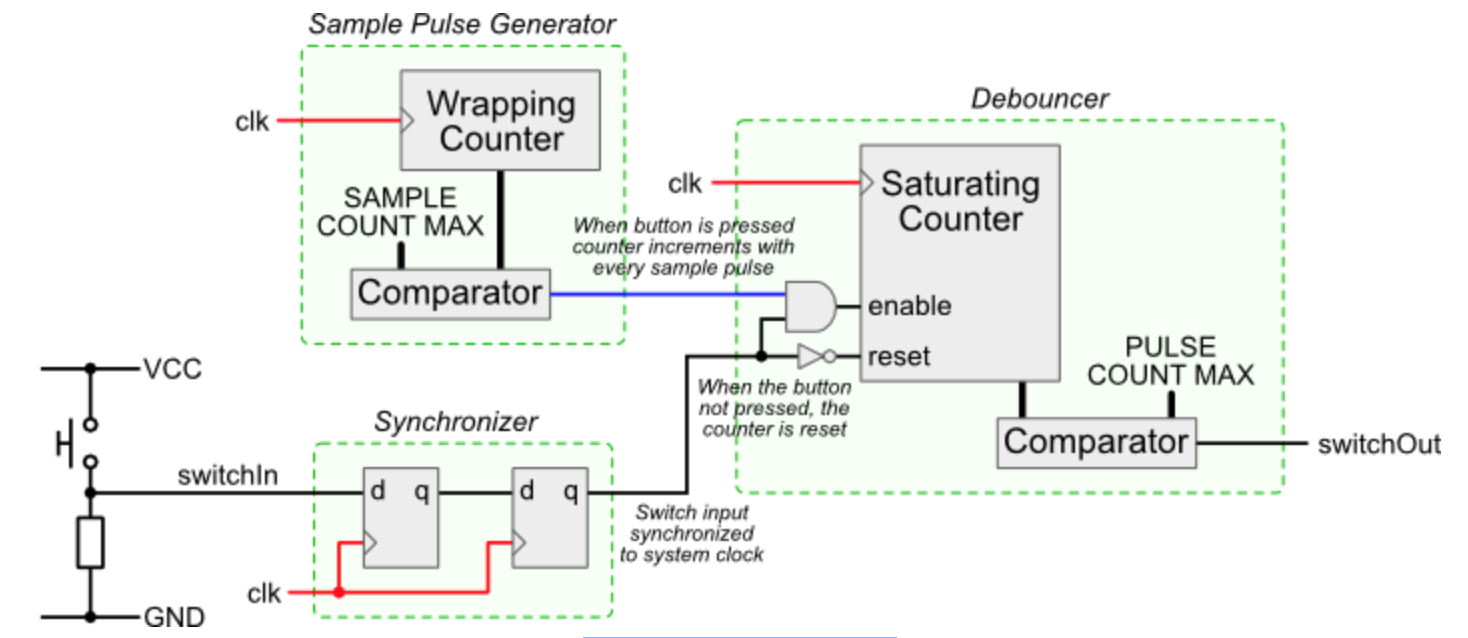
\includegraphics[height=5cm]{figs/lab2_fig2.png}}
\end{figure}

Recall this graphic from the prelab debouncer reading. It is an overview of the debouncer circuit which includes the synchronizer circuit.

For this lab, the debouncer circuit will take a button's glitchy digital input and output a clean signal indicating a single button press. The reason we need a circuit for this can be seen in the figure below.

\begin{figure}[H]
	\centerline{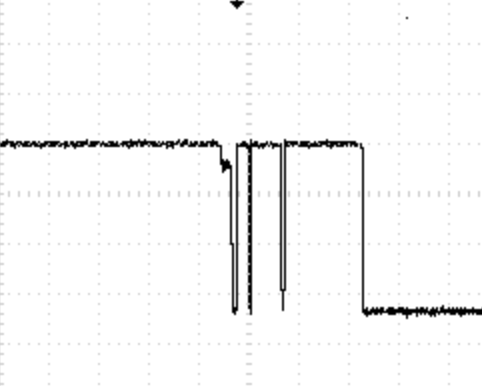
\includegraphics[height=5cm]{figs/lab2_fig4.png}}
\end{figure}

When we press the button, the signal doesn't behave like a perfect step function. Instead the button signal is glitchy due to mechanical ``bounce''. A debouncer turns this waveform, which shows a single button press, into a clean signal with a single voltage transition.

Take a look at \verb|debouncer.v| in your project sources. This is a parameterized debouncer which can debounce \verb|width| signals at a time. Your debouncer receives a vector of synchronized 1-bit signals and it outputs a debounced version of those signals. The other parameters reference the constants used in the circuit from the prelab reading.

The debouncer consists of:

\begin{enumerate}
	\item \textbf{Sample Pulse Generator} - Tells our saturating counter when to sample the input signal. It should output a 1, every \verb|sample_count_max| clock cycles. By default \verb|sample_count_max| is set to 25000.
	\item \textbf{Saturating Counter} - This is a counter that counts up to \verb|pulse_count_max|. The saturating counter should increment by one if both the sample pulse and the input signal are high at a clock edge. At any clock edge, if the input signal is 0, the saturating counter should be reset to 0. Once the saturating counter reaches \verb|pulse_count_max|, it should hold that value indefinitely until the input signal falls to 0, upon which the saturating counter should be reset to 0. The \verb|debounced_signal| of your debouncer should be an equality check between the saturating counter and \verb|pulse_count_max|.
\end{enumerate}

You should use the same sample pulse generator for all input signals into your \verb|debouncer|, but you should have a separate saturating counter per input signal. You will likely need to use a 2D reg in Verilog to create the saturating counters. You will also likely need to use generate-for.

Here is an \textbf{example} of creating a 2D array:

\begin{minted}[tabsize=4]{verilog}
reg [7:0] arr [3:0]; // 4 X 8 bit array
arr[0]; // First byte from arr (8 bits)
arr[1][2]; // Third bit of 2nd byte from arr (1 bit)
\end{minted}

And here is an \textbf{example} of using a generate-for loop:

\begin{minted}[tabsize=4]{verilog}
genvar i;
generate
	for (i = 0; i < width; i = i + 1) begin:LOOP_NAME
		always @ (posedge clk) begin
			// Insert synchronous Verilog here
		end
	end
endgenerate
\end{minted}

Implement the debouncer (in \verb|debouncer.v|).

\subsubsection{Edge Detector}

The debouncer will act to \emph{smooth-out} the button press signal. It is then followed up with an edge detector that can take the low-to-high transition of the debouncer output and use it to generate a 1 clock period wide pulse that the rest of our digital design can use.

Create a variable-width edge detector in \verb|edge_detector.v|. 

\subsubsection{Testing in Simulation}

We've provided a testbench to test your debouncer and edge detector circuits in \verb|debouncer_testbench.v| and \verb|edge_detector_testbench.v|. Run the testbench, make sure it passes, and inspect the waveforms before FPGA testing. Make sure there are no undefined (red line) signals.

If you are seeing issues where certain registers are red lines (X's), make sure you give them an initial state. For a 2D reg initialization, use the following initialization code in \verb|debouncer.v|:

\begin{minted}[tabsize=4]{Verilog}
integer k;
initial begin
	for (k = 0; k < width; k = k + 1) begin
		saturating_counter[k] = 0;
	end
end
\end{minted}

The debouncer testbench has 2 tests:
\begin{enumerate}
	\item Verifies that if a glitchy signal initially bounces and then stays high for \textbf{less} than the saturation time, that the debouncer output never goes high.
	\item Verifies that if a glitchy signal initially bounces and then stays high for \textbf{more} than the saturation time, that the debouncer goes high and stays high until the glitchy signal goes low.
\end{enumerate}

The edge detector testbench tests 2 scenarios, when the \verb|signal_in| is a pulse 10 clock cycles wide and a pulse 1 clock cycle wide and verifies that the \verb|edge_detect_pulse| output goes high twice, both times with a width of 1 clock cycle.

\subsubsection{Testing on the FPGA}
We have created a top level module called \verb|debouncer_fpga_test| that will create a 6-bit register and will use button presses to add and subtract from it. This module will use both your \verb|debouncer.v| and \verb|edge_detector.v|.

Pressing BTN1 or BTN2 will cause the register to incrment by 1. Pressing BTN0 will cause the register to decrement by 1. BTN3 resets the register to 0. The LEDs will show the current value of the register.

In your Vivado project, set \verb|debouncer_fpga_test| as the top module and run the build flow, then program the board. Make sure that you \textbf{investigate any warnings for synthesis}. You can ignore some: the top-level module has unused input/output ports to avoid having to change the XDC file. Make sure you fix any other warnings you find so that the your debouncer will work as expected on the FPGA.

You will discover when playing with your debouncer that the buttons have a way that they like being pressed to minimize bounce; get a good feel for them.


\section{Synchronous Resets In Design and Simulation}
Begin by copying your \verb|tone_generator| and \verb|music_streamer| from lab 3. \textbf{Do not change the port declaration of the lab 4 skeleton files, only copy over your implementation}.

Now that we have a debouncer that can give us a pulse for a press of a button, we have a way of explicitly resetting our circuits! You will recall that in the previous lab, we set the initial value of registers as below so that our simulation would have defined signals.

\begin{minted}[tabsize=4]{verilog}
reg [23:0] clock_counter = 0;
\end{minted}

or 

\begin{minted}[tabsize=4]{verilog}
initial clock_counter = 0;
\end{minted}

Tying one of the push buttons to a reset signal, we can now do this instead.

\begin{minted}[tabsize=4]{verilog}
always @ (posedge clk) begin
	if (rst) begin
		clock_counter <= 24'd0;
	end
	else begin
		clock_counter <= clock_counter + 24'd1;
	end
end
\end{minted}

Unlike what we did before, this Verilog is synthesizable for all deployment targets, FPGAs, ASICs, and CPLDs alike. Go ahead and modify your \verb|tone_generator| and \verb|music_streamer| to use the provided \verb|RESET| signal to get your registers to a sensible initial state.

After doing this, run the \verb|tone_generator_testbench| again using \verb|make| in the \verb|lab4/sim/| directory (or just use Vivado's simulator). View the waveform using the simulator and see how we used a reset in the testbench to bring all the registers to a defined state without specifying a default value.

\section{Music Streamer Tempo Control}
Let's use the new user inputs we now have access to. You will recall that your \verb|music_streamer| by default chooses to play each tone in the ROM for 1/25th of a second. Extend the functionality of the \verb|music_streamer| so that one input increases the tempo, one input decreases it, and one resets it to a default value. If you have the hex keypad working, you can map any of the keys to these functions, but make a note of it. If not, use the push-buttons left on the Pynq-Z1 (remembering that BTN3 is now reserved as a global reset signal).

You can implement this by using a register to hold the number of clock cycles per note. Instead of this number being hardcoded in Verilog to represent $\frac{1}{25}$th of a second, you can change it at runtime. One input should add or subtract a fixed number from this register, which should alter the time each tone is played. You get to choose this number; find something reasonable.

Try this out on the FPGA and verify that you have control of your \verb|music_streamer|'s tempo using the inputs. You should be able to speed up and slow down the music you are playing.

\section{Music Streamer FSM}
Now, you will implement a simple FSM in the \verb|music_streamer|.

The FSM will have 3 states: \verb|PAUSED|, \verb|REGULAR_PLAY|, \verb|REVERSE_PLAY|. Here is the state transition diagram:

\begin{center}
\begin{tikzpicture}[shorten >=1pt, node distance=10cm,on grid, auto]
  \tikzstyle{state} = [draw, very thick, fill=white, rectangle, minimum height=3em, minimum width=7em, node distance=17em, font={\sffamily\bfseries}]
  \tikzstyle{stateEdgePortion} = [black,thick];
  \tikzstyle{stateEdge} = [stateEdgePortion,->];
  \tikzstyle{edgeLabel} = [pos=0.5, text centered, font={\sffamily\small}];
  
	\node[state,initial](rp) {REGULAR\_PLAY};
	\node[state](revp) [below =of rp]{REVERSE\_PLAY};
	\node[state](p) [right=of rp]{PAUSED};

	\path[->]
	(rp) edge node {Play-pause button} (p)
		edge [swap] node {Reverse button} (revp)
		edge [loop above] node {} (rp)
	(p) edge node {} (rp)
		edge [loop below] node {} (p)
	(revp) edge [swap] node {Play-pause button} (p)
		edge [swap] node {} (rp)
		edge [loop below] node {} (revp);
\end{tikzpicture}
\end{center}

\begin{enumerate}
	\item Your initial state should be \verb|REGULAR_PLAY|. 
	
	\item Pressing one button should transition you into the \verb|PAUSED| state from either the \verb|REGULAR_PLAY| or \verb|REVERSE_PLAY| states. Pressing the same button while in the \verb|PAUSED| state should transition the FSM to the \verb|REGULAR_PLAY| state.
	
	\item In the \verb|PAUSED| state, your ROM address should be held steady at its value before the transition into \verb|PAUSED| and no sound should come out of the speaker. After leaving the \verb|PAUSED| state your ROM address should begin incrementing again from where it left off and the speaker should play the tones.
	
	\item You can toggle between the \verb|REGULAR_PLAY| and \verb|REVERSE_PLAY| states by using a second input button. In the \verb|REVERSE_PLAY| state you should decrement your ROM address by 1 rather than incrementing it by 1 every X clock cycles as defined by your tempo.
		
	\item If you don't press any buttons, the FSM shouldn't transition to another state.
\end{enumerate}

Your \verb|music_streamer| takes in user button inputs that it can use to transition states. If you have a working keypad you will have plenty of inputs to choose from, and you should select new inputs such that the tempo control from the previous section still works (again, remember to note your scheme). If not, you have to be creative: use an edge detector circuit with the slide switches to convert their actuation into a momentary signal (using the switch position as state would be too easy).

Also, drive the LEDs such that they show the current state. An example:

\renewcommand{\arraystretch}{1.5}
\begin{center}
\begin{tabular}{| l | l |}
	\hline
	\textbf{LED} & \textbf{Value} \\ \hline
        LEDS[5] & \verb|current_state| == \verb|REGULAR_PLAY| \\ \hline
        LEDS[4] & \verb|current_state| == \verb|PAUSED| \\ \hline
        LEDS[3] & \verb|current_state| == \verb|REVERSE_PLAY| \\ \hline
        LEDS[2:0] & 0 \\ \hline
\end{tabular}
\end{center}

You can run the testbench in \verb|music_streamer_testbench.v| to test out your state machine. Take a look at the code to see what it does and inspect your waveform to check that your FSM is performing correctly. Verify that you don't have any unexpected synthesis warnings.

Finally, program the FPGA with your \verb|music_streamer|, and verify its functionality.

\section{Checkoff}
\begin{enumerate}
  \item Prove that if the ROM contains an entry for a \verb|tone_switch_period| of 0, that the square wave doesn't oscillate.
  \item Show the working \verb|music_streamer| on the FPGA.
\end{enumerate}

\section*{Ackowlegement}
This lab is the result of the work of many EECS151/251 GSIs over the years including:
\begin{itemize}
\item Sp12: James Parker, Daiwei Li, Shaoyi Cheng
\item Sp13: Shaoyi Cheng, Vincent Lee
\item Fa14: Simon Scott, Ian Juch
\item Fa15: James Martin
\item Fa16: Vighnesh Iyer
\item Fa17: George Alexandrov, Vighnesh Iyer, Nathan Narevsky
\item Sp18: Arya Reais-Parsi, Taehwan Kim
\item Fa18: Ali Moin, George Alexandrov, Andy Zhou
\end{itemize}

\end{document}
